
\chapter{Design}

The design section of this thesis serves as a bridge between the theoretical analysis and the practical implementation of the project. This section should comprehensively outline the proposed solution, coming from the goals summarized in analysis, describing design principles, methodologies, and tools to be employed. 

\section{Goals}

First step of the design process is to summarize the goals of the project. The goals of the project are derived from the analysis section of the thesis. In subsequent subsections, the goals will serve as a base for making design decisions. 


\subsection{Compatibility with the Ataccama Expression Language}

In Ataccama, data quality rules are defined using a custom expression language Ataccama Expressions. 

The solution should be designed to be compatible with Ataccama Expressions, most importantly, a user should be able to reuse data quality rules originally written in Ataccama Expression Language, and evaluate them.

This language is defined using a formal grammar. The expected functions and operators output is defined in a separate documentation.

The goal of this project is to bring the Ataccama expression language over to Python, so that it can be executed with as little managed dependecies as possible. This means that the language will have to be implemented in such a way that it can be executed in a Python environment. To satisfy the requirement for simple configuration and ease of use, the solution should strive to avoid any additional managed dependencies, meaning any application that need to be set up outside Python dependency management, i.e. any runtimes, compilers, application. This does not apply to Python packages, which are easily managable within the Python environment itself and are a industry standard, which engineers are used to and as such satisfies the ease of use criterion. Attention must be paid to package compatibility regarding Python versions, implementations, and operating systems - requirements for this will be set later on. 


\subsection{Design an API that is easy to use for data engineers}

In the analysis section, the persona of data engineer was introduced as the main user of the solution. The main goal of the project is to design an API that is easy to use for data engineers. The API should be simple a easy to understand and use. Any complex abstraction such as advanced design patterns should be avoided. For example, the creation of object should be simple, using either a constructor or a imported function. 

Furthermore, it should be taken into account that the library will be outside of IDE and similar environments where code suggestion and documentation might not be available. For example, when writing integrations in the platforms discussed such as Azure Data Factory and Data Bricks, the user will not have access to the documentation or code suggestions. For this reason, the API should be designed to be self-explanatory, and should be designed to be easy to use without the need for extensive documentation.

\subsection{Reasonable performance}

To be considered a viable alternative to the original Ataccama implementation and to similar solutions on the market, the Python implementation should be able to handle data quality rules within Python environments efficiently and effectively. The performance of the Python implementation should be within acceptable limits, where a slowdown by a factor of up to 10 times compared to the Java version might be considered tolerable for deployment, but a 1000 times slowdown would indicate serious efficiency issues that could render the solution impractical. By establishing these performance benchmarks, we can validate that the Python implementation meets minimum requirements for real-world applications, ensuring it is a viable alternative for data engineers who require programmatic access to Ataccama's data quality tools. This will be further discussed in the evaluation section.

\section{Ataccama Expression Language}

To facilitate the integration of Ataccama's data quality rules into Python, a thorough understanding of the Ataccama Expression Language is essential. Below is an overview of the language components, types, and operational logic.

\subsection{Anatomy of an expression}

The structure of an expression in Ataccama's language consists of:

\begin{itemize}

    \item Statements
    
        \begin{itemize}
            \item Variable Assignments
            
            Variables are assigned values which can include literals, operations, or function calls.
            \item Function Definitions
            
            Optional definitions that encapsulate logic or operations reusable within the expression.
        \end{itemize}
    \item Resulting Expression
    
    This is the final part of the expression where the previously defined variables and functions are utilized to compute a result. The outcome of the resulting expression is the output of the entire expression.
\end{itemize}


\subsection{Examples of a expression}

The two following examples illustrate the structure of an expression in Ataccama's language.

\subsubsection{Simple example: Arithmetic Expression}


\begin{verbatim}
a := 10;  
b := a * 2; 
b + 5
\end{verbatim}

In this example, variables a and b are used in statements to set up values that are manipulated in the resulting expression, b + 5, which computes the final output.

\subsubsection{Complex example: Digit sum}

\begin{verbatim}
value := replace(trim(input), '-', '');
function digitSum(integer digit) { 
    set.sumExp(
        trim(substituteAll("(.)", "$1 ", toString(digit))), 
        " ", 
        (x) {toInteger(x)}
    )
}
digitSum(value) % 13 == 0
\end{verbatim}

This example demonstrates a more complex expression that includes a function definition, digitSum, which is then called in the resulting expression, digitSum(value). The expression is a simplified excerpt from a data quality rule that checks ISIN numbers for validity.

\subsection{Components of Ataccama Expression Language}

Ataccama Expression Language, also called ONE Expressions, organizes data operations and logic into a series of expressions and operands defined by a rigorous structure:


    \subsubsection{Operands}
    
    Operands in Ataccama Expressions are categorized into four main types:

    \begin{itemize}
        \item  Literals
        
        These include numeric, string, or logical constants (e.g., TRUE, FALSE) and the null literal. All keywords are case-insensitive.

        \item Columns
        
        Identified by their names, which require square brackets if they include spaces. In multiple input scenarios, columns are specified using dot notation (input\_name.column\_name). If only one input is used, dot notation can be omitted.

        \item Set
        
        Used exclusively with the IN operation, representing a constant expression. Sets can only appear on the right side of the IN operation.
    
        \item Complex Expressions
        
        These may involve various combinations of the above operand types and function calls.
    \end{itemize}

    \subsubsection{Data Types and Conversions}
    
    Operands can be of specific column types such as INTEGER, FLOAT, LONG, STRING, DATETIME, DAY, and BOOLEAN. Ataccama handles type conversions automatically, widening data types as necessary ( e.g., INTEGER - LONG - FLOAT ) to accommodate operations.

    \subsubsection{Handling Null Values}

    The handling of null values aligns with SQL rules, with a notable exception for the STRING data type. In Ataccama, a null string is considered equal to an empty string, impacting how comparisons and operations are performed.

    \subsubsection{Variables}

    Expressions in Ataccama can include sequences of assignment expressions followed by a resulting expression, separated by semicolons. The first occurrence of a variable defines its type, with subsequent references needing to conform to this type.

    \subsubsection{Operations and Functions}
    
    Ataccama ONE supports a variety of operations and functions:

    \begin{itemize}
        \item arithmetic functions
        \item logical functions
        \item comparison functions
        \item set functions
        \item date functions
        \item string functions
        \item bitwise functions
        \item MinMax functions
        \item aggregating functions
        \item conditional functions
        \item conversion functions
        \item formatting functions
        \item word set operation functions
    \end{itemize}

    The full list of functions and their descriptions can be found in the Ataccama ONE Expressions documentation \cite{one_expressions}.


\section{Architecture}

One of the first decisions to be made is the architecture of the solution.

The program itself will do the following:

\begin{enumerate}
    \item Parse the input expression
    \item Evaluate the expression on a record and return the result
\end{enumerate}

In the first step, the expression will be parsed into an abstract syntaxt tree (AST). Given the complexity of the expression language, a best-fit solution will be to use a parser generator. The parser generator will take the grammar of the language as input and generate a parser that can parse the input expression, providing a way to add custom logic into the subsequent semantic analysis of the expression.

In the semantic analysis, the AST will be traversed and built into some for of executable code so that it can be evaluated on a record. The evaluation will be done in a Python environment, and the result will be returned to the user.

In the last step, the generated code will be executed on records, and the results will be returned.

\subsection{Parser generator}

For the parser generator, a specific approach is indicated. The Ataccama Expression Language implementation uses a parser generator called ANTLR. ANTLR (ANother Tool for Language Recognition) is a powerful parser generator\cite{antlr}. It's widely used to build languages, tools, and frameworks. From a grammar, ANTLR generates a parser that can build and walk parse trees\cite{antlr4docs}. As the grammar of the Ataccama Expression Language is already defined, it is simple and robust to use adapt and reuse the grammar by also using ANTLR to generate the parser. 

\subsection{Code generation}

Having decided on the parser generator, the next step is to decide how to generate the code for the expression. There are two obvious approaches at hand: Represent the expression in an object tree with execution being a recursive descent through the tree. The second approach is to generate Python code directly. This can be done using Python standard module ast, which can be used build an abstract syntax tree of the expression, and then compile it into a Python function. Alternatively, the code can be generated as a string and then executed using Python's exec function, but this approach is less safe, more error-prone, harder to debug and introduces more overhead as it adds an additional step of parsing the code.

The second approach is more efficient, as it avoids the overhead of traversing the AST, but it is also more complex, as it requires generating Python code. The first approach might appear simpler, but it is less efficient, as it requires traversing the AST and does not include the option to use compilation to Python bytecode.

Using Python as the runtime also comes with the benefit of being able to use Python's scope resolution and name hiding to implement the scoping rules of the Ataccama Expression Language, so a reimplementation can be avoided.

For these reasons, the second approach is chosen. The code will be generated as Python code using the ast module, and then compiled into a Python module.

\section{Compatibility with the Ataccama Expression language}


The Ataccama Expression Language is complex and has many features, along with
platform specific quirks a peculiarities. For this reason, the implementation will
not be a one-to-one copy of the language, but rather a subset of the language
features that are most commonly used with some differences in behaviour.

The differences between the Ataccama Expression Language and the Python
implementation will be outlined in detail in the following sections. As the goal
is to make the implementation as close to the original language as possible, the
differences will be kept to a minimum. Consequently, the implementation will be
able to run most of the data quality rules written in the Ataccama Expression
Language.

The rest of this section describes a high level overview of the differences that
will have to be introduced along with the reasons behind them. Most of the
differences are a result of a different underlying technology, decisions have to be
made on where to draw the line between mimicking the original language and

This section has two purposes: The first is to describe the language and its features, the second is to outline and discuss design decisions related to the individual fetatures and functionality that have to be made in order to implement the language in Python 
introducing accepting differences for the sake of simplicity and performance.

\subsection{Dynamic typing}

The Ataccama Expression Language is statically typed, following its language
of implementation which is Java. This means that the type of each variable and
expression is known at compile time compile time. This allows the compiler to
catch type errors at compile time, and to generate more efficient code. Also,
it allows for function and operator overloading, as the compiler can choose the
correct function based on the types of the arguments.
This is possible thanks to the record format being known at compile time. The
record format is a schema that defines the types of the fields in the record.
Python is dynamically typed, which means that it is possible to allow for
dynamic typing in the implementation.

On the other hand, to reimplement static typing in Python would require
aditional work like keeping track of the types of all symbols and expressions and
resolving function overloads.

Furthermore, static typing would require the user to define the record format
at compile time, which would make the API less user-friendly, which in our case
is a priority. This could be solved by allowing the user to define the record format optionally.

Considering the above stated arguments, the decision is to allow for dynamic
typing in the implementation, as it is easier to implement and more flexible. 
The implementation of optional static typing is a possible future improvement, but for the initial implementation would
constitute a great effort for little gain from the user's perspective.

\subsubsection{Function and operator overloading}

The decision to utilize dynamic typing in the Python implementation of the Ataccama Expression Language carries significant implications for function and operator overloading. Unlike in Java, where Ataccama's static typing enables the compiler to select the correct function or operator based on argument types at compile time, Python's dynamic typing means the types of variables are only known at runtime. This characteristic prevents overloading functions and operators based on type, as there is no way to determine the type of the inputs beforehand.

As a result, each function in the Python implementation must be universally applicable, handling all expected input types through internal logic. This requires implementing comprehensive type checking within each function, where the function determines the appropriate action based on the runtime types of the arguments. Such an approach aligns with Python’s duck typing philosophy, where operations are attempted regardless of type, with the function internally managing any type mismatches or errors. This method ensures flexibility and broad applicability of functions, albeit at the cost of the type-specific optimization possible in statically typed languages like Java.

\subsection{Implementation scope}

The Ataccama Expression Language supports over 150 functions but the implementation in Python will be limited to a subset of
the language features. The reasoning behind this is that many of the functions are
not commonly used, and the implementation of all of them would be a significant
effort and would be out of scope for this project as the goal is to provide a simple
prototype and validate the viability first. 

For this reason, the functions have been categorized by priority, and the implementation will
focus on the high- and medium-priority functions. The categorization is based on the frequency of use of the tasks in the data quality rules, and the complexity of the implementation. The high-priority functions are the most commonly used functions, and the medium-priority functions are less commonly used but still important. 
The prioritization comes from Ataccama's knowledge base. The low-priority functions are the least commonly used functions, and will not be implemented in the initial version of the implementation. 

A list of all function along with their priority and implementation status can be found in the appendix \ref{app:list-of-functions}.


\subsection{Arithmetic}
The Ataccama Expression Language operates, like standard types in Java, in
fixed-size bit arithmetic, i.e., 32 bits for integers and 64 bits for Python. 
On the other hand, Python uses arbitrary precision arithmetic, which means that the size
of the integers is not limited. This means that the results of arithmetic operations
can differ between the two languages.
For everyday operations, the difference is not significant, and it could be said
that the Python behaviour is better. However, in some use cases, the fixed-size
arithmetic is necessary, for example, when working with hash tables. As the number
of these cases is limited and most of them are provided as implemented functionality,
the implementation will use Python-native arbitrary precision arithmetic and
handle fixed-size arithmetic as a special case where necessary.

Furthermore, the Ataccama Expression Language provides arithmetic operators
for addition, subtraction, multiplication, division, integer division, and remainder. 
Python provides the same operators, but
the behaviour of the operators is different. The first significant difference
is the handling of null values. In Ataccama Expression Language, the operators are null safe and
follow a SQL-like behaviour. In Python, the operators throw an exception if any of the operands is null.
Also, the arithmetics are different; modulo and division produce different results for negative operands. These differences will have to be addressed as the
results differ too much to be ignored.  Moreover, Python uses arbitrary precision arithmetic, whereas Ataccama Expressions use the underlying Java types, but this difference is not significant for most use cases and could be considered an improvement. 
Lastly, the plus operator in Ataccama Expression Language is overloaded for string concatenation, converting any non-string to string first, which is not the case in Python. This will have to be implemented as it is a common use case.


\subsection{Null handling and null coalescing}

The way Ataccama Expression language handles nulls has a lot of aspects
which have to be addressed.

Operators handle null values in a SQL-like way, mostly returning null if any
of the operands is null. The implication for the implementation is that it will not be
possible to use native Python operators, as they do not handle null values in the
same way.

Empty strings are treated as null values. The documentation states: "A null
string and an empty string are considered equal". Moreover, in the Ataccama Expression Language, most empty string
returns are coalesced to null. This behaviour also has its own quirks, for example
‘1 + null == null‘ but ‘1 + "" == "1"‘, which breaks the aforementioned statement.

Furthermore, functions have to be prepared to handle null values in any of the
arguments. Most commonly, functions return null if any of the arguments is null,
so extensive null checking has to be implemented in the functions.
The implementation in Python will have to address these differences and
provide a way to handle null values in a Python environment.
Date and floating point formatting

\section{Interface design}

There are not a lot of decisions to be made in the API Design as the public
functionality is simple. The following diagram shows the public interface of the transpiler.

\begin{figure}[htbp]
    \centering
    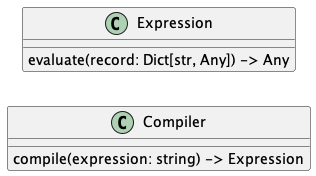
\includegraphics[scale=0.7]{diagrams/api_design-class.png}
    \caption{API overview}
    \label{fig:api}
\end{figure}


The functionality is simple and so is the interface.  All necessary actions are to compile an expression and run it. 


